% ### Uses XeLaTeX ### %
% ### Needs beamer-master ### %
\documentclass[aspectratio=169]{beamer} %. Aspect Ratio 16:9
\usetheme{AI2} % beamerthemeSprace.sty
% DATA FOR FOOTER
\date{2019}
\title{}
\author{}
\institute{Advanced Institute for Artificial Intelligence (AI2)}
\begin{document}    
% ####################################
% FIRST SLIDE 						:: \SliTit{<Title of the Talk>}{<Author Name>}{<Intitution>}
% SLIDE SUB-TITLE					:: \SliSubTit{<Title of the Chapter>}{<Title of the Section>}
% SLIDE WITH TITLE 					:: \SliT{<Title>}{Content}
% SLIDE NO TITLE 						:: \Sli{<Content>} 
% SLIDE DOUBLE COLUMN WITH TITLE 	:: \SliDT{<Title>}{<First Column>}{<Second Column>}
% SLIDE DOUBLE COLUMN NO TITLE 		:: \SliD{<First Column>}{<Second Column>}
% SLIDE ADVANCED WITH TITLE 			:: \SliAdvT{<Title>}{<Content>}
% SLIDE ADVANCED  NO TITLE 			:: \SliAdv{<Content>}
% SLIDE ADVANCED DOUBLE TITLE 		:: SliAdvDT{<Title>}{<First Column>}{<Second Column>}
% SLIDE ADVANCED DOUBLE NO TITLE 	:: SliAdvD{<First Column>}{<Second Column>}
% ITEMIZE 							:: \begin{itemize}  \IteOne{1st Level} \IteTwo {2nd Level} \IteThr{3rd Level} \end{itemize}
% SECTION 							:: \secx{Section} | \secxx{Sub-Section}
% COLOR BOX 						:: \blu{blue} + \red{red} + \yel{yellow} + \gre{green}
% FRAME 							:: \fra{sprace} \frab{blue} \frar{red} + \fray{yellow} + \frag{green}	
% REFERENCE						:: \refer{<doi number>}
% FIGURE 							::  \img{X}{Y}{<scale>}{Figures/.png} 
% FIGURE							:: \begin{center}\includegraphics[scale=<#>]{Figures/.png}\end{center}
% PROJECT STATUS					:: \planned\~    \started\~   \underway\~   \done\~   
% EXERCICIO							:: \Exe{<#>}{<text>}
% STACKREL							:: \underset{<down>}{<up>}
% FLUSH LEFT						:: \begin{flalign*}  & <1st equation> & \\  & <12nd equation>  & \\ \end{flalign*}
% REAL / IMAGINAY					:: \Re / \Im
% SLASH								:: \sl{} or \sl
% BOLD MATH							:: \pmb{<>}
% ####################################
%
% FIRST SLIDE :: DO NOT BREAK LINE !!!
\SliTit{Python}{Advanced Institute for Artificial Intelligence}{https://advancedinstitute.ai}

% SLIDE WITH TITLE
\SliT{Sumario}{

\begin{itemize}
  \IteOne{Introdução}
  \IteOne{Estruturas e Função de Controle}
  \IteOne{Coleções}
  \IteOne{Programação Orientada a Objetos}
  \IteOne{Manipulação de arquivos}
  \IteOne{Processos e Threading}  
\end{itemize}

}

% SLIDE WITH TITLE
\SliT{Introdução}{

\begin{itemize}
  \IteOne{Python é uma linguagem interpretada}
  \IteOne{Caminho do Python no Sistema}
  \IteTwo{which python}
  \IteOne{Versão do Python}
  \IteTwo{python -V}

\end{itemize}

}





% SLIDE WITH TITLE
\SliT{Usando Python}{

\begin{itemize}
  \IteOne{Iniciando interpretador Python}
  \IteTwo{python}
  \IteTwo{Python 3.6.8 |Anaconda, Inc.| (default, Dec 30 2018, 01:22:34) }
  \IteTwo{[GCC 7.3.0] on linux}
  \IteTwo{Type "help", "copyright", "credits" or "license" for more information.}
  \IteTwo{$>>>$ Esse é o prompt para receber comandos python }
  \IteOne{Ctrl+D sai do interpretador }
\end{itemize}

}

% SLIDE WITH TITLE
\SliT{Usando Python}{

Comando print

\begin{itemize}
  \IteOne{print "hello world"}
  \IteTwo{Em python 2 é possível utilizar dessa forma:}
  \IteOne{print "hello world"}
  \IteTwo{Em python 3 é obrigatório utilizar $($ $)$}
  \IteOne{print ("hello world")}
\end{itemize}

Comentários no código
\begin{itemize}
  \IteOne{\# : comentando uma linha}
  \IteOne{''' : começar e terminar bloco de comentário}
  \IteOne{""" : começar e terminar bloco de comentário}
\end{itemize}

}

% SLIDE WITH TITLE
\SliT{Usando Python}{

Indentação

\begin{itemize}
  \IteOne{O controle de início e fim deblocos de código é feito por meio de Indentação}
  \IteOne{Indentação pode ser controlada por um tamanho fixo de espaços em branco}
  \IteOne{Exemplo}
  \IteTwo{print ("teste")}
  \IteTwo{if (i == 0):}
  \IteTwo{\hspace{1cm} print ("0")}
  \IteTwo{else:}
  \IteTwo{\hspace{1cm} print ("outro valor")}
  \IteTwo{\hspace{1cm} if (i $>$= 0):}
  \IteTwo{\hspace{2cm} print ($>$=0")}

\end{itemize}


}
% SLIDE WITH TITLE
\SliT{Tipos de dados - Números}{

Existem três tipos numéricos em python: números inteiros, números de ponto flutuante e números complexos. 

\begin{itemize}
  \IteOne{Booleanos são um subtipo de números inteiros. }
  \IteOne{Inteiros têm precisão ilimitada.}
  \IteOne{Números de ponto flutuante são geralmente implementados usando tipo Double em C}
\end{itemize}

}

\SliT{Tipos de dados - Strings}{

Strings podem ser manipuladas de diversas maneiras em Python

\begin{itemize}
  \IteOne{podem ser representadas usando aspas simples ' ' ou aspas duplas " "  }
  \IteOne{É possível utilizar catacteres escape   }

\end{itemize}

}


\SliT{Funções}{

\begin{itemize}
  \IteOne{A palavra-chave def é usada para definir funções}
  \IteOne{Deve ser definida antes de ser utilizada}
  \IteOne{O valor de retorno padrão é None}
\end{itemize}

}

\SliT{Função}{
Argumento pode ser gerado da seguinte forma:
\begin{itemize}
  \IteOne{nome de variável}
  \IteOne{nome de variável e tipo padrão}
\end{itemize}

Escopo de variável
\begin{itemize}
  \IteOne{variáveis possuem escopo local ao bloco onde são criadas}
  \IteOne{Pode ser definidas variáveis globais}
\end{itemize}

}

\SliT{Funções}{

Função sem argumentos:
\hfill \break
\hfill \break
def greeting():

\hspace{1cm} print("hello world")

\hfill \break
\hfill \break
greeting()

}

\SliT{Argumento de Função}{

def numsquare(num):

\hspace{1cm} return num * num

\hfill \break
number=10
\hfill \break
numsquare(number)

\hfill \break
def numsquare(num=10):

\hspace{1cm} return num * num

\hfill \break
numsquare()

}

\SliT{Obtendo dados do usuário}{

função input() é utilizada para aguardar um valor digitado no terminal pelo usuário.
\hfill \break
\hfill \break
usrip = input("número inteiro: ")
\hfill \break
usrnum = int(usrip)
\hfill \break
sqrnum = numsquare(usrnum)
\hfill \break
print("Square of entered number is: {}".format(sqrnum))
\hfill \break
\hfill \break
usrip = input("float: ")
\hfill \break
usrnum = float(usrip)
\hfill \break
sqrnum = numsquare(usrnum)
\hfill \break
print("Square of entered number is: {}".format(sqrnum))
\hfill \break
\hfill \break
usrname = input("nome: ")
\hfill \break
print("nome: ",usrname)

}
\SliT{Usando bibliotecas adicionais}{

A palavra reservada import permite adicionar pacotes que não são nativos do Python
\hfill \break
\hfill \break
import subprocess
\hfill \break
\# Executa um comando linux no terminal
\hfill \break
subprocess.call('date')
\hfill \break
\hfill \break
A palavra reservada from premite importar apenas parte de um pacote 
\hfill \break
\hfill \break
exemplo:
\hfill \break
\hfill \break
from sklearn.model\_selection import train\_test\_split
}

\SliT{Estruturas e Função de Controle}{

Argumento pode ser gerado da seguinte forma:
\begin{itemize}
  \IteOne{if}
  \IteOne{for}
  \IteOne{while}
\end{itemize}

}

\SliT{Estruturas e Função de Controle}{

if 
\begin{itemize}
  \IteOne{As instruções if avaliam uma condição, caso seja verdadeira executa o bloco seguinte}
  \IteOne{Pode ser combinado com uma estrutura else, que é executada quando a condição não é verdadeira no bloco if}
\end{itemize}

Exemplo:

var = 100
\hfill \break
if (var==100):

\hspace{1cm} print("100")
\hfill \break
else: 
\hspace{1cm} print("not 100")

}

\SliT{Estruturas e Função de Controle}{

for
\begin{itemize}
    \IteOne{executam um certo bloco de código para um número conhecido de iterações. }
    \IteOne{Um bloco de código pode ser executado para o número de itens existentes em uma lista, dicionário, variável de sequência ou tupla}
    \IteOne{Um bloco de código pode ser executado em um intervalo contado de etapas}
\end{itemize}

Exemplo:
\hfill \break

a=(10,20,30,40,50)
\hfill \break
for b in a:
\break
\hspace{1cm} print "square of " + str(b) + " is " +str(b*b)

}

\SliT{Estruturas e Função de Controle}{

while

\begin{itemize}
    \IteOne{O loop while é executado enquanto uma declaração condicional retorna true }
    \IteOne{A instrução condicional é avaliada toda vez que um bloco de código é executado }
    \IteOne{A execução para no momento em que a instrução condicional retorna false. }
\end{itemize}

Exemplo:
\hfill \break

count = 0
\hfill \break
while (count $<$ 9):
    \hfill \break
    \hfill \break
    \hspace{1cm} print("iteração",count)
    \hfill \break
    \hspace{1cm} count+=1


}


\SliT{Coleções}{

Uma coleção nos permite colocar muitos valores em uma única "variável"

Uma coleção é útil para transportar valores em um único pacote.

friends = [ 'Joseph', 'Glenn', 'Sally' ]

carryon = [ 'socks', 'shirt', 'perfume' ]

Coleções em python:

list, set, stack, dictionary, tuplas, entre outros

}

\SliDT{List}{

Os elementos na lista (list) são separados por vírgulas.

Um elemento da lista pode ser qualquer objeto Python - até outra lista

Uma lista pode estar vazia

Operador index representa uma posição na lista
}{
list = [1, 24, 76]

list = ['red', 'yellow', 'blue']

list = ['red', 24, 98.599999999999994]

list = [1, [5, 6], 7]

l[0] =$>$ 1
}

\SliT{List}{

Listas são mutáveis

lotto = [2, 14, 26, 41, 63]

print lotto

[2, 14, 26, 41, 63]

lotto[2] = 28

print lotto

[2, 14, 28, 41, 63]

Operador \textbf{len} retorna tamanho da lista

print len(lotto)

5
}


\SliT{List}{

\textbf{Append} adiciona elementos no fim da lista

Operador \textbf{in} pode ser usado para verificar se um elemento existe na lista

\textbf{sort} classifica a lista

\textbf{split} quebra uma string em partes menores usando estrutura de lista
}

\SliT{Dicionários}{

Dicionários são estruturas que mapeiam chaves para valores

Operações: 

print, del, len, in

Métodos: 

keys(), values(), items()

}

\SliT{Dicionários}{

eng2sp = ${}$

Adicionando valores

$>>>$ eng2sp['one'] = 'uno'

$>>>$ eng2sp['two'] = 'dos'

declarando dicionário com valores iniciais

$>>>$ eng2sp = [] 'one': 'uno', 'two': 'dos', 'three':'tres' ]

}



\SliT{List Comprehensions}{

Aplica uma expressão a cada elemento da lista

vec = [2, 4, 6]

$>>>$ [3*x for x in vec]

    [6, 12, 18]

$>>>$ [3*x for x in vec if x > 3]

    [12, 18]

}

\begin{comment}
\SliT{Tupla}{

uma sequência ordenada de elementos, pode misturar tipos de elementos
não pode alterar os valores dos elementos (imutável)

}
\end{comment}

\SliT{Slicing}{

Listas podem ser filtradas por meio de 'slicing' 

Formato para realizar 'slicing' em uma lista: s[start:end:step]

Elementos:

\begin{itemize}
    \IteOne{s: um objeto que pode ser manipulado por 'slicing' }
    \IteOne{start: primeiro índice para iniciar a iteração }
    \IteOne{end: último indíce, NOTE que o índice final não será incluído na fatia resultante }
    \IteOne{step: escolha o elemento a cada índice de etapa }
\end{itemize}


}

\SliT{Slicing}{

Alguns Exemplos:

\begin{itemize}
    \IteOne{Selecionar itens a partir do índice start até stop-1 }
    \IteTwo{a[start:stop] }
    \IteOne{Selecionar itens a partir do índice start até o final }
   \IteTwo{a[start:] }
    \IteOne{Selecionar itens a partir do início start até stop-1 }
    \IteTwo{a[:stop] }
    \IteOne{Copia toda a lista }
    \IteTwo{a[:] }

\end{itemize}
}

\SliT{Slicing}{

Alguns Exemplos:

\begin{itemize}
    \IteOne{Selecionar itens a partir do índice start não passando de stop-1, realizando pulos definidos na variável step}
    \IteTwo{a[start:stop:step]}
    \IteOne{Último item da lista}
    \IteTwo{a[-1] }   
    \IteOne{Últimos dois itens da lista}
    \IteTwo{a[-2:] }  
    \IteOne{Tudo menos os dois úlitmos}
    \IteTwo{a[:-2]  } 
\end{itemize}
}

\SliT{Slicing}{

Alguns Exemplos:

\begin{itemize}
    \IteOne{Quando a lista possuir mais de uma dimensão, é necessário realizar o slicing separadamente em cada dimensão}
\end{itemize}

\begin{itemize}
    \IteOne{Apagando elementos de uma lista}
    \IteTwo{del a[3:7]  } 
\end{itemize}

}

\SliT{Manipulação de Texto}{

Abrir um arquivo:

\begin{itemize}
    \IteOne{Preparar o arquivo para leitura:}
    \IteOne{Vincula a variável do arquivo ao arquivo físico   } 
    \IteOne{Posiciona o ponteiro do arquivo no início do arquivo.   } 
\end{itemize}

Formato: 
     $<$variável do arquivo$>$ = open ($<$nome do arquivo$>$, "r")

Exemplo:
    inputFile = open ("data.txt", "r")
    
    filename = input ("Digite o nome do arquivo de entrada:")
    
    inputFile = open (filename, "r")
}

\SliT{Manipulação de Texto}{

Comando para fechar um arquivo

Formato:

$<$name of file variable$>$.close()

Exemplo:

inputFile.close()

}

\SliT{Manipulação de Texto}{

Normalmente, a leitura é feita dentro do corpo de um loop

Cada execução do loop lê uma linha do arquivo em uma string

Formato:

for $<$variável para armazenar uma sequência$>$ em $<$nome da variável do arquivo$>$:

    $<$Faça algo com a string lida no arquivo$>$

Exemplo:

for line in inputFile:
    print (line) 

}


%\SliT{Manipulação de Texto}{

%Escrita de arquivo

%Exemplo 1:

%f = open("f.txt", "w")

%f.write("teste")

%f.close()    

%Exemplo 2:

%with open("new_file.txt", "w") as f:

%    f.write("This is a sample line of text\n")
    
%    f.write("Yet another line\n")

%}


\SliT{Orientação a objeto}{

Orientação a Objetos surgiu da necessidade de modelar sistemas complexos

\begin{itemize}
    \IteOne{Modelar problemas utilizando um conjunto de componentes autocontindo, e integráveis}
    \IteOne{Determinar como um objeto deve se comportar e como deve interagir com outros objetos}
\end{itemize}

Algumas iniciativas:

\begin{itemize}
    \IteOne{Simula 67 (60)}
    \IteOne{Smalltalk (70)}
    \IteOne{C++ (80)}
\end{itemize}

}

\SliT{Orientação a objeto}{

Conceitos essenciais:
\begin{itemize}
    \IteOne{Classes e objetos}
    \IteOne{Atributos e Métodos}
    \IteOne{Herança}
    \IteOne{Encapsulamento}
\end{itemize}

}

\SliT{Orientação a objeto}{

Os objetos reais possuem duas caracterísicas:

\begin{itemize}
    \IteOne{Estado (Atributos)}
    \IteOne{Comportamento}
\end{itemize}

Exemplos:
\begin{itemize}
    \IteOne{cachorro}
    \IteTwo{Estado: nome, cor, raça}
    \IteTwo{Comportamento: latindo, abanando o rabo, comendo}
\end{itemize}

}

\SliT{Orientação a objeto}{

Um objeto de software é conceitualmente similar aos objetos reais

\begin{itemize}
    \IteOne{Objetos armazenam seu estado em atributos}
    \IteTwo{Correspondentes às variáveis em programação estruturada.}

    \IteOne{Objetos expõem seu comportamento através de métodos}
    \IteTwo{Correspondentes às funções em programação estruturada.}
\end{itemize}

}


\SliT{Orientação a objeto}{

Exemplos de objeto:

\begin{itemize}
    \IteOne{Gerenciador de Dados de Alunos}
    \IteTwo{Estado: lista de alunos}
    \IteTwo{Comportamento: filtrar alunos por nome, incluir aluno, alterar aluno}
\end{itemize}

\begin{itemize}
    \IteOne{Biblioteca Matemática}
    \IteTwo{Estado: Matriz }
    \IteTwo{Comportamento: calcular transposta, multiplicar, somar }
\end{itemize}

}

\SliT{Orientação a objeto}{

Empacotar o código em objetos individuais fornece:
\begin{itemize}
    \IteOne{Modularidade }
    \IteTwo{Objetos são independente}
    \IteOne{Encapsulamento }
    \IteTwo{Os detalhes da implementação de um objeto permanecem ocultos}
    \IteOne{Reuso }
    \IteTwo{Objetos podem ser reutilizados em diferentes programas}
    \IteOne{Fraco acoplamento }
    \IteTwo{Objetos podem ser substituídos facilmente}
\end{itemize}

}

\SliT{Orientação a objeto}{

Uma classe é o projeto a partir do qual objetos individuais são criados

\begin{itemize}
    \IteOne{Ela define os atributos e os métodos correspondentes aos seus objetos. }
    \IteOne{Outros possíveis membros de uma classe são:}
    \IteTwo{Construtores: define as operações a serem realizadas quando um objeto é criado.}
    \IteTwo{Destrutores: define as operações a serem realizadas quando um objeto é destruído.}
\end{itemize}

}

\SliT{Orientação a objeto}{

Outras características de uma classe:

\begin{itemize}
    \IteOne{Uma classe pode herdar características de outra classe e incluir novas características}
    \IteOne{Atributos de uma classe podem ser protegidos, sendo possível alterar seu conteúdo por meio apenas de métodos da própria classe}
    \IteOne{Métodos podem ser reescritos}
\end{itemize}

}

\SliT{Orientação a objeto}{

\begin{itemize}
    \IteOne{O relacionamento de Herança define um relacionamento do tipo generalização}
    \IteOne{Indica que uma classe (subclasse) é especializada para gerar uma nova (superclasse)}
    \IteOne{Tudo que a superclasse possui, a subclasse também vai possuir}
    \IteOne{Em Python, todas as classes herdam a classe Object}
\end{itemize}

}


\begin{frame}[fragile] \frametitle{Orientação a objeto}

\begin{center}
    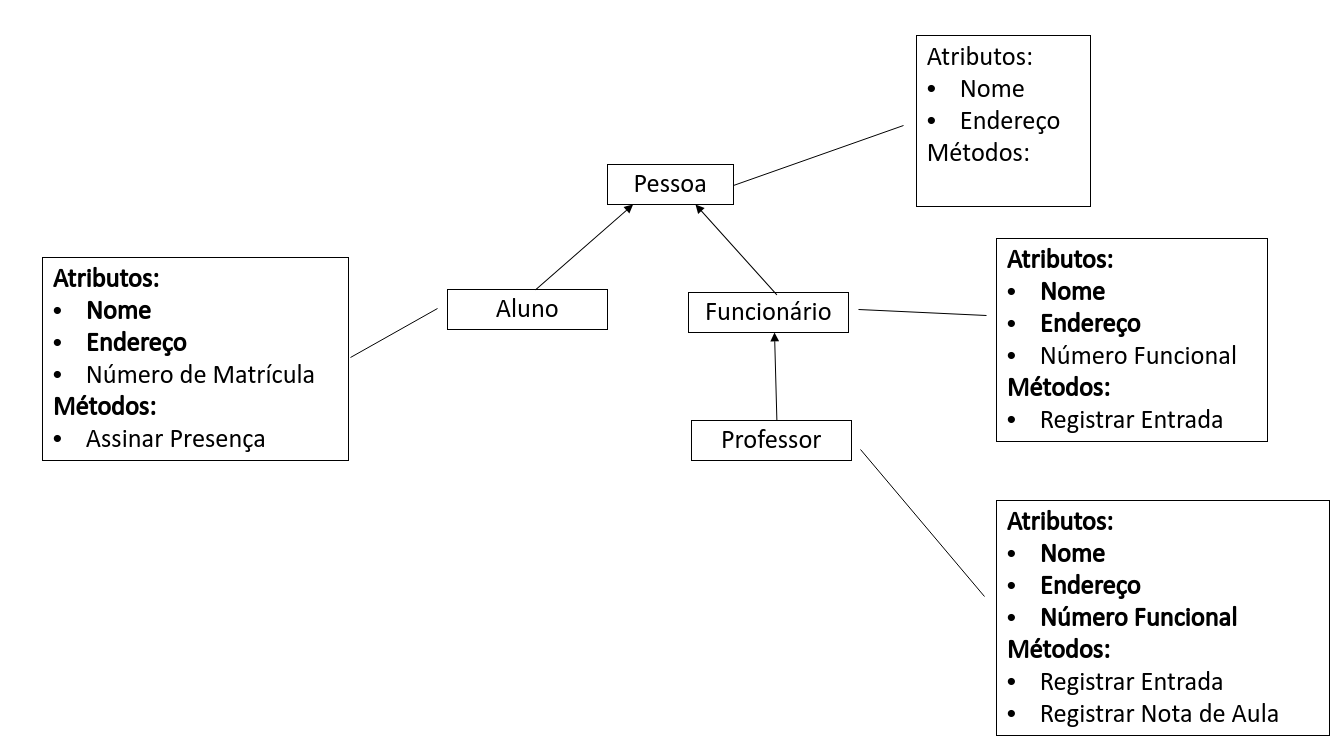
\includegraphics[scale=0.27]{heranca1.png}     
    \end{center}
}

\end{frame}

\begin{frame}[fragile] \frametitle{Orientação a objeto}
Método Construtor em Python

\begin{verbatim}
def __init__(self):
    Comandos do construtor
    
\end{verbatim}


Parâmetro para referenciar ao objeto criado: self

self.name cria uma variável name e associa ao objeto criado.

\begin{verbatim}
class Critter:
    def __init__(self, name):
        self.name = name
\end{verbatim}

\end{frame}

\begin{frame}[fragile] \frametitle{Orientação a objeto}

Para definir Métodos Privados em Python é necessário incluir: \begin{verbatim}__\end{verbatim}

Exemplo:
\begin{verbatim}
__a 
__my_variable
\end{verbatim}

Para definir que Classe deve herdar outra Classe, deve se colocar o nome da classe a ser herdade entre (), logo após o nome da classe:

\begin{verbatim}
class teste(object):
    def __init__(self, X):
        self.X = X
\end{verbatim}


\end{frame}

\begin{frame}[fragile] \frametitle{Orientação a objeto}

Exemplo de uma classe em Python
\begin{verbatim}
class MyClass:
    def function(self):
        print("This is a message inside the class.")
\end{verbatim}

Instanciando um objeto e chamando métodos:
\begin{verbatim}
myobjectx = MyClass()
myobjectx.function()
\end{verbatim}

\end{frame}


\begin{frame}[fragile] \frametitle{Orientação a objeto}

Exemplo de uma classe em Python
\begin{verbatim}
# Classe que representa uma coordenada X Y
class Coordinate(object):
    #define um construtor
    def __init__(self, x, y):
        # configura coordenada x e y
        self.x = x
        self.y = y
    #reimplementa a função __str__    
    def __str__(self):
        # Representação em string da coordenada
        return "<" + str(self.x) + "," + str(self.y) + ">"
\end{verbatim}

\end{frame}

\begin{frame}[fragile] \frametitle{Orientação a objeto}

\begin{verbatim}
def distance(self, other):
    # Calcula distancia euclidiana entre dois pontos
    x_diff_sq = (self.x-other.x)**2
    y_diff_sq = (self.y-other.y)**2
    return (x_diff_sq + y_diff_sq)**0.5
\end{verbatim}

Teste de Uso da Classe
\begin{verbatim}
c = Coordinate(3,4)
origin = Coordinate(0,0)
print("Coordenada 1:")
print(c)
print(c.distance(origin))
\end{verbatim}

\end{frame}

\begin{frame}[fragile] \frametitle{Orientação a objeto}
Teste com atributos protegidos

\begin{verbatim}
class MyClass:
    __variable = 0
    def setvariable(self,newvar):
        self.__variable = newvar
    def getvariable(self):
        return (self.__variable)
    def function(self):
        print("This is a message inside the class.")
\end{verbatim}

\end{frame}

\begin{frame}[fragile] \frametitle{Orientação a objeto}
Teste com atributos protegidos

\begin{verbatim}
var="rs2"
myobjectx = MyClass()
myobjectx.function()
print(myobjectx.getvariable())
var="rs3"
myobjectx.setvariable(var)
print(myobjectx.getvariable())
\end{verbatim}

\end{frame}

\SliT{Criando Pacotes para Compartilhamento de Classes}{

}

\SliT{MultiThreading}{

}

\end{frame}

\end{document}